\chapter{Long-baseline Neutrino Oscillation Physics}
\label{ch:physics-lbnosc}

\section{Context}
\label{sec:physics-lbnosc-context}

{\bf [Note: Copied from Section 2.2 of the LBNE Science Document.]}  
The Standard Model of particle physics 
presents a remarkably accurate
description of the elementary particles and their
interactions. However, its limitations beg deeper questions about
Nature. The unexplained patterns of quarks, leptons, flavors and
generations imply that a more fundamental underlying theory must
exist.  
DUNE plans to pursue a detailed
study of neutrino mixing, resolve the neutrino mass ordering,
and search for CP violation in the lepton sector by
studying the oscillation patterns of high-intensity
$\nu_\mu$ and $\overline{\nu}_\mu$ beams measured over a long baseline. 
Neutrino oscillation arises from mixing between the flavor and mass eigenstates of neutrinos,
corresponding to the weak and gravitational interactions, respectively. 
This three-flavor-mixing
scenario can be described by a rotation between the weak-interaction
eigenstate basis $(\nu_e,\, \nu_\mu,\, \nu_\tau)$ and the basis of
states of definite mass $(\nu_1,\, \nu_2,\, \nu_3)$.  In direct
correspondence with mixing in the quark sector, the transformations
between basis states is expressed in the form of a complex unitary
matrix, known as the PMNS matrix :
\begin{equation}
\left(\begin{array}{ccc} \nu_e \\ \nu_\mu \\ \nu_\tau \end{array} \right)= 
\underbrace{
  \left(\begin{array}{ccc}
      U_{e 1} &  U_{e 2} & U_{e 3} \\ 
      U_{\mu1} &  U_{\mu2} & U_{\mu 3} \\ 
      U_{\tau 1} &  U_{\tau 2} & U_{\tau 3} 
    \end{array} \right)
}_{U_{\rm PMNS}} \left(\begin{array}{ccc} \nu_1 \\ \nu_2 \\ \nu_3 \end{array} \right).
\label{eqn:pmns0}
\end{equation}
The PMNS matrix in full generality depends on just three mixing angles
and a CP-violating phase.  The mixing angles and phase are designated
as $(\theta_{12},\, \theta_{23},\, \theta_{13})$ and
\deltacp.  %\fixme{mathmatical rep of mixing}
This matrix can be parameterized as the product of three
two-flavor mixing matrices as follows, where $c_{\alpha \beta}=\cos \theta_{\alpha \beta}$ and $s_{\alpha
  \beta}=\sin \theta_{\alpha \beta}$:

\begin{equation}
U_{\rm PMNS} = 
  \underbrace{
    \left( \begin{array}{ccc}
        1 & 0 & 0 \\ 
        0 & c_{23} & s_{23} \\ 
        0 & -s_{23} & c_{23}
    \end{array} \right)
  }_{\rm I}
\underbrace{
  \left( \begin{array}{ccc}
      c_{13} & 0 & e^{i\delta_{cp}}s_{13} \\ 
      0 & 1 & 0 \\ 
      -e^{i\delta_{cp}}s_{13} & 0 & c_{13}
  \end{array} \right) 
}_{\rm II}
\underbrace{
 \left( \begin{array}{ccc}
      c_{12} & s_{12} & 0 \\ 
      -s_{12} & c_{12} & 0 \\ 
      0 & 0 & 1
  \end{array} \right) 
}_{\rm III}
\label{eqn:pmns}
\end{equation}
The parameters of the PMNS
matrix determine the probability amplitudes of the neutrino
oscillation phenomena that arise from mixing.  The frequency of neutrino oscillation 
depends on the difference in the squares of the neutrino
masses, $\Delta m^{2}_{ij} \equiv m^{2}_{i} - m^{2}_{j}$; a set of three
neutrino mass states implies two independent mass-squared differences
($\Delta m^{2}_{21}$ and $\Delta m^{2}_{32}$). The ordering of the
mass states is known as the \emph{neutrino mass hierarchy}. An ordering of
$m_1 < m_2 < m_3$ is known as the \emph{normal hierarchy} since it matches
the ordering of the quarks in the Standard Model, whereas an ordering of $m_3 < m_1 < m_2$
is referred to as the \emph{inverted hierarchy}.

The entire complement of neutrino experiments to date has measured
five of the mixing parameters: the three angles $\theta_{12}$,
$\theta_{23}$ and (recently) $\theta_{13}$, and the two mass differences
$\Delta m^{2}_{21}$ and $\Delta m^{2}_{32}$. The sign of $\Delta
m^{2}_{21}$ is known, but not that of $\Delta m^{2}_{32}$, which 
is the crux of the 
mass hierarchy ambiguity.
The values of $\theta_{12}$ and $\theta_{23}$ are large, while 
$\theta_{13}$ is smaller~\cite{An:2012bu}. The value of \deltacp is unknown.
The real values of the entries of the PMNS mixing matrix, which
contains information on the strength of flavor-changing weak decays in
the lepton sector, can be expressed in approximate form as

\begin{equation}
|U_{\rm PMNS}|\sim \left(\begin{array}{ccc} 0.8 & 0.5 & 0.2 \\ 0.5 & 0.6 & 0.6 \\ 0.2 & 0.6 & 0.8\end{array} \right).
\label{eq:pmnsmatrix}
\end{equation}

%\fixme{math rep of comparison of nu to Q}

The three-flavor-mixing scenario for neutrinos is now well
established. However, the mixing parameters are not known to the same precision 
as are those in the
corresponding quark sector, and several important quantities, including
the value of \deltacp and the sign of the large mass splitting, are
still undetermined. In addition, several recent
anomalous experimental results count among their possible
interpretations phenomena that do not fit this 
model~\cite{Aguilar:2001ty,AguilarArevalo:2007it,Aguilar-Arevalo:2013pmq,Mention:2011rk}.

The relationships between the values of the parameters in the neutrino
and quark sectors suggest that mixing in the two sectors is
qualitatively different. Illustrating this difference, the value of
the entries of the CKM quark-mixing matrix (analogous to the PMNS matrix for
neutrinos, and thus indicative of the strength of flavor-changing weak
decays in the quark sector) can be expressed in approximate form as
\begin{equation}
|V_{\rm CKM}|\sim \left(\begin{array}{ccc} 1 & 0.2 & 0.004\\ 0.2 & 1 & 0.04 \\ 0.008 & 0.04 & 1\end{array} \right)
\label{eq:ckmmatrix}
\end{equation}
and compared to the entries of the PMNS matrix given in Equation~\ref{eq:pmnsmatrix}.
As discussed in \cite{King:2014nza}, the question of why the quark mixing angles are
smaller than the lepton mixing angles is an important part of the ``flavor problem.''

Quoting the discussion in~\cite{deGouvea:2013onf}, ``while the CKM
matrix is almost proportional to the identity matrix plus
hierarchically ordered off-diagonal elements, the PMNS matrix is far
from diagonal and, with the possible exception of the $U_{e3}$
element, all elements are ${\cal O}(1)$.''
One theoretical method often used to address this question involves the use of non-Abelian discrete
subgroups of $SU(3)$ as flavor symmetries; the popularity of this method comes partially from
the fact that these symmetries can give rise to the nearly \emph{tri-bi-maximal}\footnote{Tri-bi-maximal mixing refers to a form of the neutrino mixing matrix with effective bimaximal mixing of $\nu_\mu$ and $\nu_\tau$
at the atmospheric scale ($L/E \sim$ \SI{500}{\km / \GeV}) and effective trimaximal
mixing for $\nu_e$ with $\nu_\mu$ and $\nu_\tau$ 
at the solar scale ($L/E \sim$ \SI{15000}{\km / \GeV})~\cite{Harrison:2002er}.} 
structure of the PMNS matrix.
Whether employing these flavor symmetries or other methods,
any theoretical principle that attempts to describe the fundamental
symmetries implied by the observed organization of quark and neutrino
mixing --- such as those proposed in unification models --- leads to
testable predictions such as sum rules between CKM and PMNS
parameters~\cite{deGouvea:2013onf,Mohapatra:2005wg,King:2014nza,Albright:2006cw}.
Data on the patterns of neutrino mixing 
are already proving crucial in the quest for a 
relationship between quarks and leptons and their seemingly arbitrary generation
structure.  
%Table~\ref{tab:params} displays the comparison between quark and lepton mixing
%in terms of the fundamental parameters 
% and the precision to which they are known\footnote{A global fit~\cite{Fogli:2012ua} to 
%  existing results from current
%  experiments sensitive to neutrino oscillation effects is the source for the PMNS matrix values.}, 
% highlighting the limited precision  of the neutrino-mixing parameter measurements.

% \begin{table}[!htb]
% \caption[Best-fit values of the neutrino mixing parameters in the PMNS
%   matrix]{Best-fit values of the neutrino mixing parameters in the PMNS
%   matrix (assumes normal hierarchy) from~\cite{Fogli:2012ua}, their $1\sigma$ uncertainties and comparison to 
% the analogous values in the CKM
%  matrix~\cite{Beringer:1900zz}. $\Delta M^2$ is defined as $m_3^2
% - (m_1^2+m_2^2)/2$.}
% \begin{center}
% \begin{tabular}[!htb]{$L^c^c}
% \toprule
% \rowtitlestyle
% Parameter  & Value (neutrino PMNS matrix) & Value (quark CKM matrix)\\
% \toprowrule
% \rowstyle{\normalfont}
% 
% $\theta_{12}$     & $34 \pm 1^{\circ}$ & $13.04 \pm 0.05^{\circ}$\\ 
% \colhline
% $\theta_{23}$     & $38 \pm 1^{\circ}$ & $2.38 \pm 0.06^{\circ}$\\ 
% \colhline
% $\theta_{13}$     & $8.9 \pm 0.5^{\circ}$  & $0.201 \pm 0.011^{\circ}$\\ 
% \colhline
% $\Delta m^2_{21}$  & $+(7.54 \pm 0.22) \times 10^{-5}$ eV$^2$ & \\ 
% \colhline
% $|\Delta M^2|$    & $(2.43^{+0.10}_{-0.06}) \times 10^{-3}$ eV$^2$ & $m_3 >> m_2$\\ 
% \colhline
% $\mdeltacp$  & $-170 \pm 54^{\circ}$ &  $67 \pm 5^{\circ}$\\
% \bottomrule
% \end{tabular}
% \end{center}
% \label{tab:params}
% \end{table}
%

Clearly much work remains in order to complete the standard three-flavor 
mixing picture, particularly 
with regard to $\theta_{23}$ (is it less than, greater than, or equal
to $45^\circ$?), mass hierarchy (normal or inverted?) 
and \deltacp. %(the value is unconstrained at the $2\sigma$ level by the global fit).  SAID ON NEXT PAGE 
Additionally, there is 
great value in obtaining a set of measurements for multiple parameters 
\emph{from a single experiment}, so that correlations and systematic 
uncertainties can be handled properly.  Such an experiment would also be 
well positioned to extensively test the standard picture of three-flavor mixing.  
DUNE is designed to be this experiment.

\section{Expected Event Rate and Sensitivity Calculations}

The oscillation probability of \numu $\rightarrow$ \nue through matter, 
to first order, in a constant density
approximation is~\cite{Nunokawa:2007qh}:
%
\begin{eqnarray}
\label{eq:oscprob}
P(\nu_\mu \rightarrow \nu_e) & \simeq & \sin^2 \theta_{23} \sin^2 2 \theta_{13} 
\frac{ \sin^2(\Delta_{31} - aL)}{(\Delta_{31}-aL)^2} \Delta_{31}^2\\ \nonumber
& & + \sin 2 \theta_{23} \sin 2 \theta_{13} \sin 2 \theta_{12} \frac{ \sin(\Delta_{31} - aL)}{(\Delta_{31}-aL)} \Delta_{31} \frac{\sin(aL)}{(aL)} \Delta_{21} \cos (\Delta_{31} + \delta_{CP})\\ \nonumber
& & + \cos^2 \theta_{23} \sin^2 2 \theta_{12} \frac {\sin^2(aL)}{(aL)^2} \Delta_{21}^2, \\ \nonumber
\end{eqnarray}
%
where 
  \[ \Delta_{ij} = \Delta m^2_{ij} L/4E,\ {\rm and} \ a=G_F N_e /\sqrt{2}. \]
%
In the above, both \deltacp and $a$ 
switch signs in going from the
$\nu_\mu \to \nu_e$ to the $\overline{\nu}_\mu \to \overline{\nu}_e$ channel; i.e.,
a neutrino-antineutrino asymmetry is introduced both by the CP-violating
phase, \deltacp, and the matter effect, the origin of which 
is simply the presence of electrons and absence of positrons in the Earth.  
The asymmetry from the matter effect increases with baseline as the neutrinos
pass through more matter, so an experiment with a longer baseline will be
more sensitive to the neutrino mass hierarchy. For baselines longer than 
$\sim$1200~km {\bf [Note: Can we provide a reference?]}, the degeneracy between the asymmetries from matter
and CP-violation effects can be resolved, so DUNE, with a baseline of 1300~km, 
will be able to unambiguously
determine the neutrino mass hierachy and measure the value of \deltacp in the same experiment.

The electron neutrino appearance probability, $P(\nu_\mu \rightarrow \nu_e)$, 
is shown in 
Figure \ref{fig:oscprob} 
at a baseline of 1300~km as a function of neutrino 
energy for several values of \deltacp. As this figure illustrates, the value 
of \deltacp affects both the amplitude and frequency of
the oscillation. The difference in probability amplitude
for differing values of \deltacp is larger at higher oscillation nodes, which 
correspond to energies less than 1.5~GeV. Therefore, a broadband experiment, 
capable of measuring not only the rate of \nue appearance but of mapping out the 
spectrum of observed oscillations down to energies of at least 500~MeV, 
is desirable. Since there are terms proportional to $\sin\delta_{cp}$ in Eq.~\ref{eq:oscprob},
changes to the value of \deltacp induce opposite changes to \nue and
\anue appearance probabilities, so a beam that is capable of operating in
neutrino (forward horn current) and antineutrino (reverse horn current)
is also a critical component of the experiment.

\begin{figure}[!htbp]
\centering
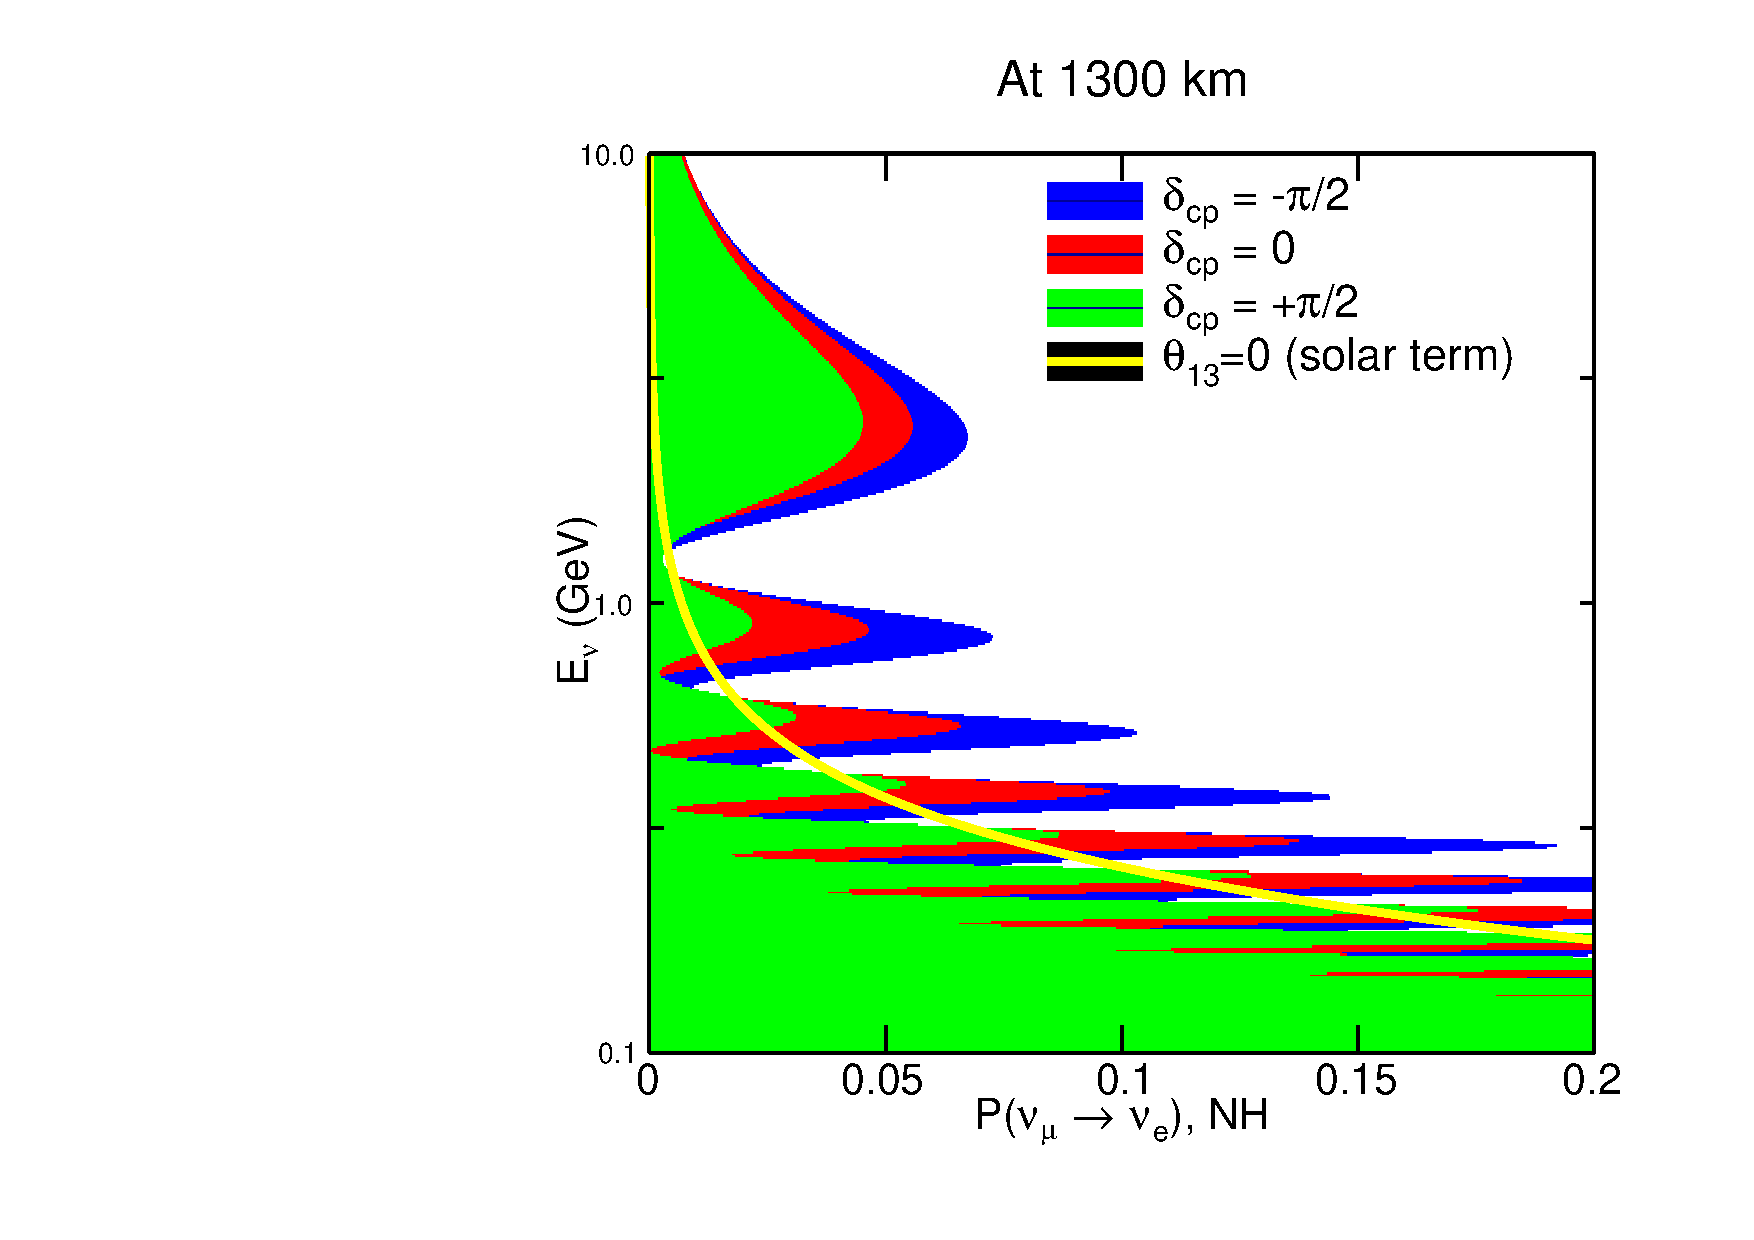
\includegraphics[width=0.45\linewidth]{energy_nu_no.pdf}
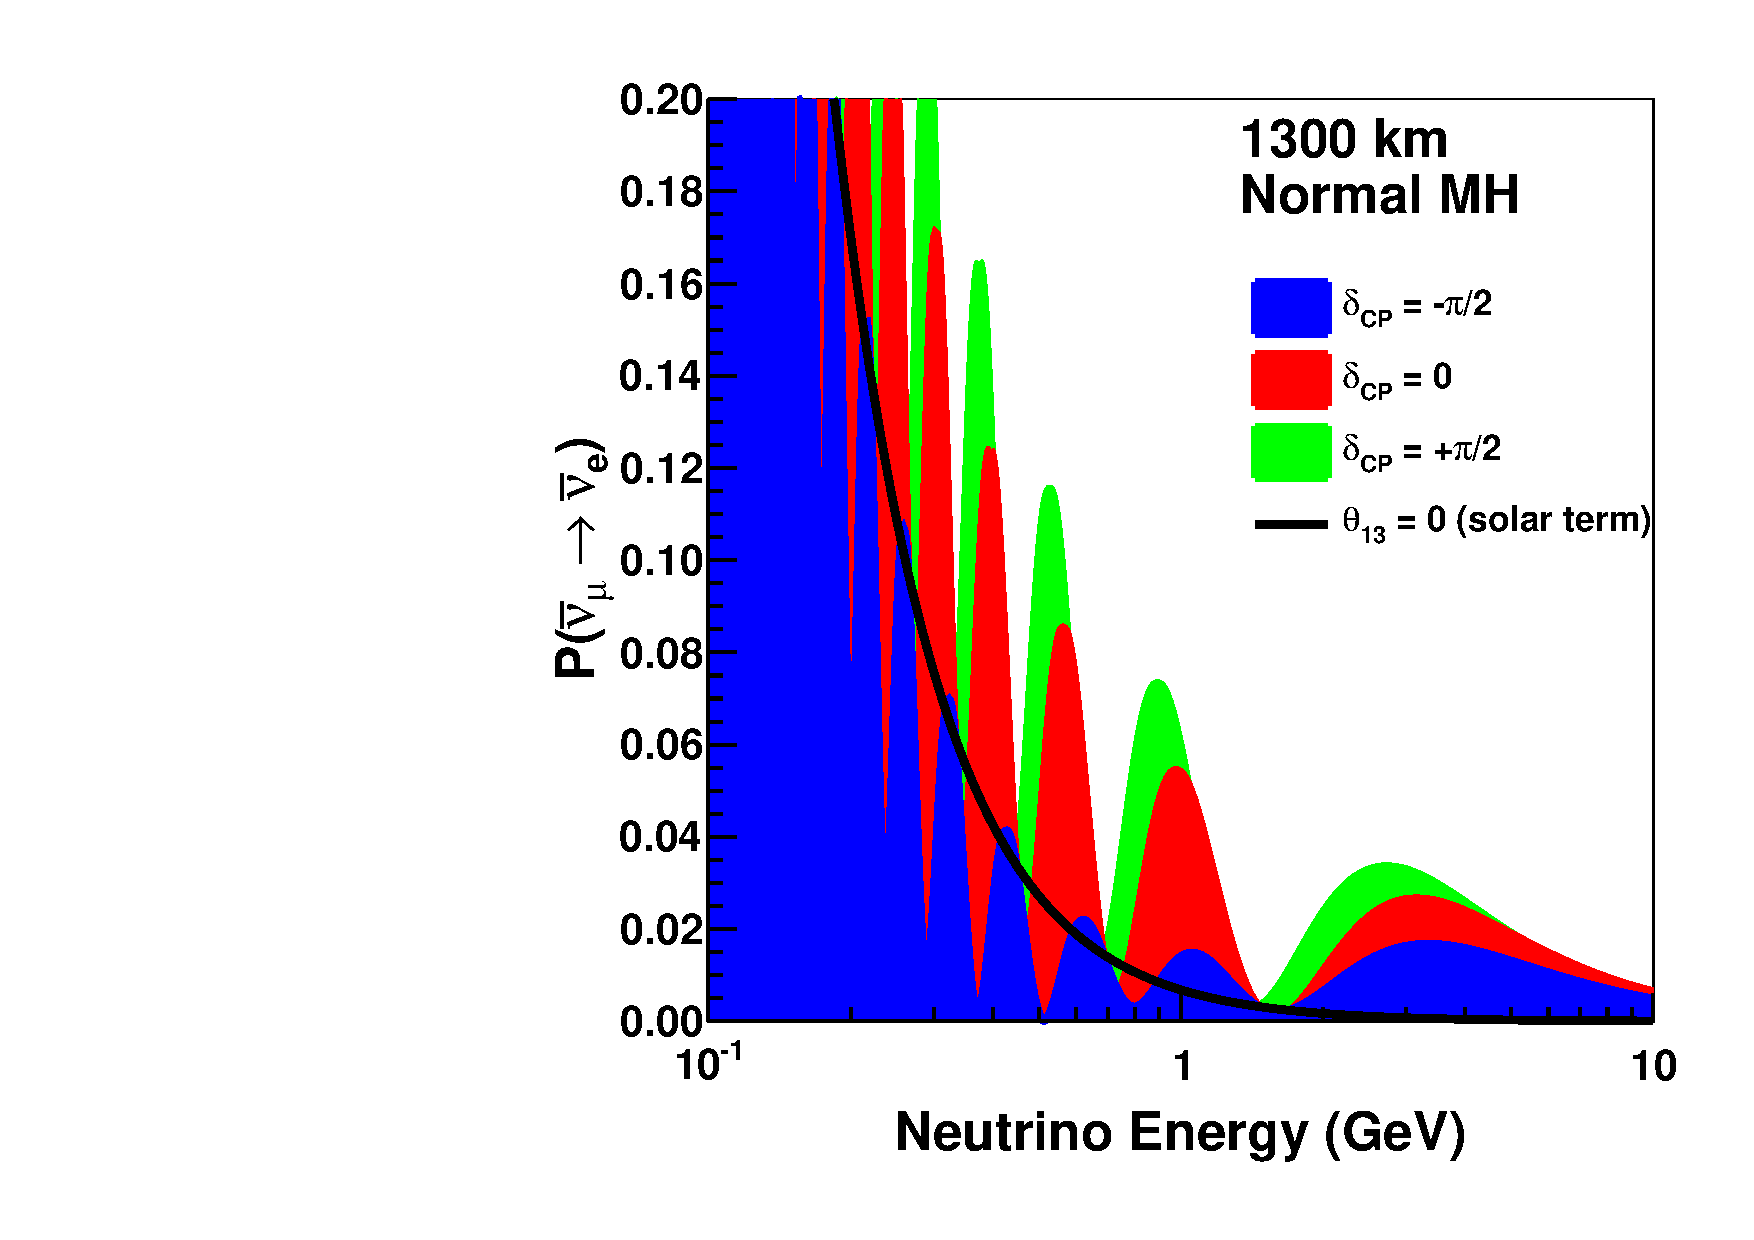
\includegraphics[width=0.45\linewidth]{energy_anu_no.pdf}
\caption{$P(\nu_\mu \rightarrow \nu_e)$ at a baseline of 1300~km,
  as a function of neutrino energy, for \deltacp = $-\pi/2$ (blue), 
  0 (red), and $\pi/2$ (green), for neutrinos (left) and antineutrinos
  (right), for normal hierarchy. The yellow line indicates the oscillation
  probability if $\theta_{13}$ were equal to zero.}
\label{fig:oscprob}
\end{figure}

The experimental sensitivities presented here are estimated using 
GLoBES\cite{globes1,globes2}. GLoBES takes flux simulation, cross-sections,
and detector-response parameterization as inputs. In this document we present
a range of possible experimental performance that depends on the design of the neutrino beam.
A conservative estimate of sensitivity is calculated using a flux simulation that is based on the reference design of the beam line as presented in {\bf [How to reference LBNF design?]}.  A flux simulation based on an optimized beam design is used to show the goal sensitivity.  There are a range of design options that produce sensitivities in between the sensitivity of the reference beam design and optimized beam design. The actual flux will depend upon details of the hadron production and focusing design; optimization of the beam design to maximize experimental sensitivity is a critical aspect of the experiment
design.  Section~\ref{sec:physics-lbnosc-beam-req} describes the flux simulations used for the sensitivity estimates and explores the possible improvements that could be achieved by variations in the reference beam design.


The LAr TPC performance parameters that go into the GLoBES calculation are generated using a fast Monte Carlo (MC) simulation, described in detail in \cite{lbne_sciencebook}.  The MC uses flux simulations and the GENIE event generator \cite{Andreopoulos:2009rq} to generate neutrino interactions on argon.  Events can then be classified as $\nu_e$ CC-like or background-like based on event-level reconstructed quantities.   {\bf [Add more details of classification?]}
% The detector response assumed in these calculations
% is summarized in Table~\ref{tab:lar-nuosc-totaltable}. 
The energy smearing, signal efficiency, and misidentification rates for background vary with energy. {\bf [How to succinctly summarize energy-dependent quantities? Efficiency and resolution at first osc max?]} The neutrino oscillation
parameters and the uncertainty on those parameters are taken from the 
Nu-Fit\cite{Gonzalez-Garcia:2014bfa} global fit to neutrino data; the values are given in 
Table~\ref{tab:oscpar_nufit}.  The cross-section inputs to GLoBES have been generated using GENIE 2.8.4~\cite{Andreopoulos:2009rq}.

% \begin{table}[!hb]
% \begin{center}
% \caption{LArTPC detector performance parameters assumed in GLoBES sensitivity
%   calculations. Signal efficiencies, background levels, and resolutions are 
%   obtained from ICARUS results and LArSoft simulations. {\bf TO BE UPDATED}}
% \label{tab:lar-nuosc-totaltable}
% \begin{tabular}{l|c} \hline\hline
% Parameter &    Value Used for  DUNE Sensitivities\\ \hline\hline
% & For $\nu_e$ CC appearance studies: \\ 
% $\nu_e$ CC efficiency          & 80\%   \\ 
% $\nu_\mu$ NC mis-identification rate  & 1\%   \\ 
% $\nu_\mu$ CC mis-identification rate  & 1\%   \\ \hline
% & For $\nu_\mu$ CC disappearance studies: \\ 
% $\nu_\mu$ CC efficiency          & 85\%   \\ 
% $\nu_\mu$ NC mis-identification rate  & 1\%   \\ 
% Other background                 & 0\% \\ \hline
% & Neutrino energy resolutions: \\ 
% $\nu_e$ CC energy resolution & $15\%/\sqrt{E(GeV)}$ \\ 
% $\nu_\mu$ CC energy resolution & $15\%/\sqrt{E(GeV)}$ \\ 
% \end{tabular}
% \end{center}
% \end{table}

\begin{table}[!hb]
\begin{center}
\caption{Central value and relative uncertainty of neutrino oscillation 
  parameters from a global fit to neutrino oscillation data, for normal hierarchy. 
  The relative uncertainty is computed using 1/6 of the 3$\sigma$ allowed range from
  the fit.}
\label{tab:oscpar_nufit}
\begin{tabular}{l|c|c} \hline\hline
Parameter &    Central Value & Relative Uncertainty \\ \hline \hline
$\theta_{12}$ & 0.5843 & 2.3\% \\
$\theta_{23}$ & 0.738  & 5.9\% \\
$\theta_{13}$ & 0.148  & 2.5\% \\
$\Delta m^2_{21}$ & 7.5$\times10^{-5}$ eV$^2$ & 2.4\% \\
$\Delta m^2_{31}$ & 2.457$\times10^{-3}$ eV$^2$ &  2.0\% \\
\end{tabular}
\end{center}
\end{table}
%

%

Figure {\bf To be added}
% %~\ref{fig:event_spec}
shows the expected event rate, including
expected flux, cross-section, and oscillation probabilities as a function 
of neutrino energy for a 40-kt fiducial mass LAr TPC at a baseline of 1300~km. 
{\bf [Description of plot.  Add rate table.]}
As illustrated in Fig.~\ref{fig:event_spec}, collection of
a large sample of \nue appearance and \numu disappearance 
events covering a broad range of energies with significant statistics at the energy
of the second oscillation maximum is possible.

%
% \begin{figure}[!htbp]
% \centering
% \includegraphics[width=0.45\textwidth]{figs/Nu_60GevPerfect_3yrs.pdf}
% \includegraphics[width=0.45\textwidth]{figs/ANu_60GevPerfect_3yrs.pdf}
% \includegraphics[width=0.45\textwidth]{figs/60GeVPerfect_3yrs_nu_dis.pdf}
% \includegraphics[width=0.45\textwidth]{figs/60GeVPerfect_3yrs_anu_dis.pdf}
% \caption{The  expected reconstructed 
%   neutrino energy spectrum of $\nu_e$ appearance (top) and \numu disppearance (bottom)
%   events in a 40-kt fiducial mass LArTPC for three years of neutrino (left) and
%   three years of antineutrino (right) running with a 1.03-MW, 60-GeV perfect focus beam.
%   The number of expected signal plus background events is shown for 
%   $\dcp = -\pi/2$, 0, and $\pi/2$. Spectra are for normal hierarchy.}
% \label{fig:event_spec}
% \end{figure}

Sensitivity to determination of the neutrino mass hierarchy and discovery
of CP violation are obtained by
simultaneously fitting the $\nu_\mu \rightarrow \nu_\mu$,
$\overline{\nu}_\mu \rightarrow \overline{\nu}_\mu$, $\nu_\mu \rightarrow \nu_e$, 
and  $\overline{\nu}_\mu \rightarrow \overline{\nu}_e$ oscillated spectra.  We assume 50\% of the total exposure comes in neutrino beam mode and 50\% in antineutrino beam mode.  Small deviations from a 1:1 ratio of neutrino to antineutrino data have been shown to have a minimal effect on the senstivity {\bf [Cite something?]}
An example of the \nue appearance and \numu disappearance spectra is shown in 
Fig.~\ref{fig:event_spec}.
The background to \nue appearance is composed of: i) intrinsic \nue and \anue 
from the beam; ii) mis-identified \numu and \anumu CC events; 
iii) neutral current (NC) backgrounds; iv) $\nu_\tau$ and $\bar{\nu}_\tau$ CC events 
in which the $\tau$'s decay leptonically into electrons/positrons. NC and $\nu_\tau$ 
backgrounds are due to interactions of higher energy neutrinos but they contribute to 
backgrounds mainly at low energy, which is important for the sensitivity to CP violation. 
Compared to the number of events shown in Figure {\bf xx}, an optimization of the beam, 
reducing the high energy tail of the flux, will help in significantly reducing this 
background. 
% As shown in \cite{::2013kaa}, $\nu_\tau$ interactions 
% have a different energy-missing 
% momentum distribution compared to the signal events and with appropriate cuts, which have
% not yet been included in this analysis, this background can be significantly reduced. {\bf(More on reduction of tau background? plots?)}

The neutrino oscillation parameters are all
allowed to vary, constrained by a Gaussian prior with 1$\sigma$ width given
by the relative uncertainties shown in Table~\ref{tab:oscpar_nufit}.
The effect of systematic uncertainty
is approximated using signal and background normalization uncertainties, which
are treated as 100\% uncorrelated among the four samples.
% Unless otherwise stated, the goal uncertainties of 1\% on signal normalization 
% and 5\% on background normalization for the \nue and \anue
% appearance measurements, in conjunction with uncorrelated
% 5\% signal and 10\% background normalization uncertainties in the \numu and
% \anumu disappearance measurements, are used to calculate the sensitivities.
The baseline systematic uncertainty estimates and the effect
of considering larger signal and background normalization uncertainties are
discussed in Section~\ref{sec:physics-lbnosc-beamnd-req}. 

In these fits, experimental sensitivity is
quantified using a test statistic, $\Delta\chi^2$, which is calculated
by comparing the predicted spectra for alternate hypotheses.
These quantities are defined, differently for neutrino mass hierarchy
and CP violation sensitivity, to be:
\begin{eqnarray}
\Delta\chi^2_{MH} & = & \chi^2_{IH} - \chi^2_{NH}\textrm{ (true normal hierarchy),}\\ 
\Delta\chi^2_{MH} & = & \chi^2_{NH} - \chi^2_{IH}\textrm{ (true inverted hierarchy),}\\
\Delta\chi^2_{CPV} & = & Min[\Delta\chi^2_{CP}(\delta_{CP}^{test}=0),\Delta\chi^2_{CP}(\delta_{CP}^{test}=\pi)]\textrm{, where} \\
\Delta\chi^2_{CP} & = & \chi^2_{\delta_{CP}^{test}} - \chi^2_{\delta_{CP}^{true}}. \\ \nonumber
\end{eqnarray}
Since the true value of $\delta_{CP}$ is unknown, a scan is  performed over
all possible values of $\delta_{CP}^{true}$. 
We define a ``typical experiment'' as one with the most probable data given a set of input parameters, 
i.e. in which no statistical fluctuations have been applied.
In this case, the predicted spectra and the true spectra are identical;
for the example of CP violation, $\chi^2_{\delta_{CP}^{true}}$ 
is identically zero and the $\Delta\chi^2_{CP}$ value for a typical experiment is given by 
$\chi^2_{\delta_{CP}^{test}}$.
{\bf [Add octant chi2, calculation of resolutions.]}

\section{Mass Hierarchy}
\label{sec:physics-lbnosc-mh}

Physics of MH (very brief).

The value of the test statistic for a typical experiment,  
$\overline{\Delta\chi^2}$, is
representative of the mean or the most likely value of $\Delta\chi^2$ that 
would be obtained in an ensemble of experiments.
With the exception of Figure~\ref{fig:mhstats}, the sensitivity plots
in this document have been generated using this method.
However, to address the expected sensitivity of a future experiment
requires consideration of the effect of
statistical fluctuations and variations in systematics.  If the
experiment is repeated many times, a distribution of $\Delta\chi^2$
values will appear.  Studies in~\cite{Qian:2012zn,Blennow:2013oma}
show that, in the case of the mass hierarchy
determination, the $\Delta \chi^2$ metric
{\em does not} follow the commonly expected chi-squared
function for one degree of freedom, which has a mean of
$\overline{\Delta\chi^2}$ and can be interpreted using a Gaussian
distribution with a standard deviation of
$\sqrt{|\overline{\Delta\chi^2}|}$. Rather, these studies show that
when the observed counts in the experiment are large enough,
the distribution of $\Delta\chi^2$ used here approximately follows
a Gaussian distribution with a
mean and standard deviation of $\overline{\Delta\chi^2}$ and
$2\sqrt{|\overline{\Delta\chi^2}|}$, respectively. Figure {\bf [Like Fig 4 of LOI]}
shows the range of sensitivity to the neutrino mass hierarchy, 
for the nominal exposure of 257 kt-MW-years,
when statistical
fluctuations are included and the statistical power as a function of exposure
for 3$\sigma$ and 5$\sigma$ sensitivity. 
% \begin{figure}[!htbp]
% \centering
% \includegraphics[width=0.45\linewidth]{figs/NHdeltacp.pdf}
% \includegraphics[width=0.45\linewidth]{figs/NHpower.pdf}
% \caption{Sensitivity to neutrino mass hierarchy including statistical fluctuations.
%   Expected sensitivity of DUNE to determination of the neutrino mass
%   hierarchy for a 40-kt fiducial mass LAr TPC and an 80-GeV, 1.07-MW beam from FNAL to SURF
%   with three years of running in neutrino and three years in antineutrino mode. 
%   {\bf Left:} The 
%   sensitivity, given by  $\sqrt{\Delta T}=\sqrt{\Delta\chi^2}$, for a typical experiment 
%   (solid blue line) is compared to the bands within which
%   68\% (green) and 95\% (yellow) of experiments are expected to fall. The dashed lines
%   represent the value of the $\Delta T$ metric above which the minimum
%   probability of determining
%   the correct neutrino mass hierarchy is 50\%(cyan), 98.9\% (blue), or $1 - 3.7\times10^{-6}$
%   (black). The red line shows the minimum sensitivity for a typical 
%   experiment.
%   {\bf Right:} The test power ($p= 1-\beta$), which represents the probability of accepting
%   the correct (NH) hypothesis, while excluding the incorrect (IH) hypothesis at the 
%   3$\sigma$ and 5$\sigma$ level, shown as a function of exposure in kt-MW-years. The width
%   of the bands represent the range of \deltacp values.
%   Sensitivities are for true normal hierarchy.}
% \label{fig:mhstats}
% \end{figure}

MH results: nominal MH sensitivity, MH sensitivity vs exposure, MH sensitivity vs theta23, MH sensitivity vs theta13, MH sensitivity vs deltam2, MH vs real time (i.e. staging)???  Table: required exposure for 5sigma 100\% coverage for reference and optimized beams.

\section{CP-symmetry Violation}
\label{sec:physics-lbnosc-cpv}

Physics of CPV measurement (brief).

CPV results: nominal CPV sensitivity, CPV sensitivity vs exposure, CPV sensitivity vs theta23, CPV sensitivity vs theta13, CPV sensitivity vs deltam2, CPV vs real time (i.e. staging)???. Table: required exposure for 3sigma 75\% coverage and 5sigma 50\% coverage for reference and optimized beams.

\section{Precision Oscillation Parameter Measurements}

Octant sensitivity, resolution for delta, theta13, theta23, deltam2

\section{Testing the 3-flavour Paradigm}
\label{sec:physics-lbnosc-3nutests}

NSI, include reference NSI plot in science document.  Sterile neutrinos.  No plots.

\section{Neutrino Beam Requirements}
\label{sec:physics-lbnosc-beam-req}

\subsection{Reference Design Focusing System}
\label{subsec:reference-design-focusing-system}
The reference beam design described in Volume 3 includes targetry and
focusing horns similar to those currently in operation in the NuMI
beamline~\cite{numitdr}, but slightly modified to accomodate a 1.2 MW primary proton beam.  The
target is composed of 47 graphite fins, each 2 cm long x 10 mm wide x
15 mm tall, and begins 45 cm upstream of the first focusing horn.  The separation
of the upstream faces of the two horns is 6.6 m.  Neutrino fluxes for the reference beam are
shown in Figure~\ref{fig:beam_req_reference_flux}.  Changes to
parameters such as the position of the target can be used to produce substantially different neutrino
energy spectra, as demonstrated in Figure~\ref{fig:beam_req_lemehe}.

\begin{cdrfigure}[Neutrino fluxes for the reference focusing 
  system.]{beam_req_reference_flux}{Neutrino fluxes for the reference 
    focusing system operating in neutrino mode (left) and antineutrino 
    mode (right).} 
\centering 
\begin{minipage}{0.45\textwidth}
\centering 
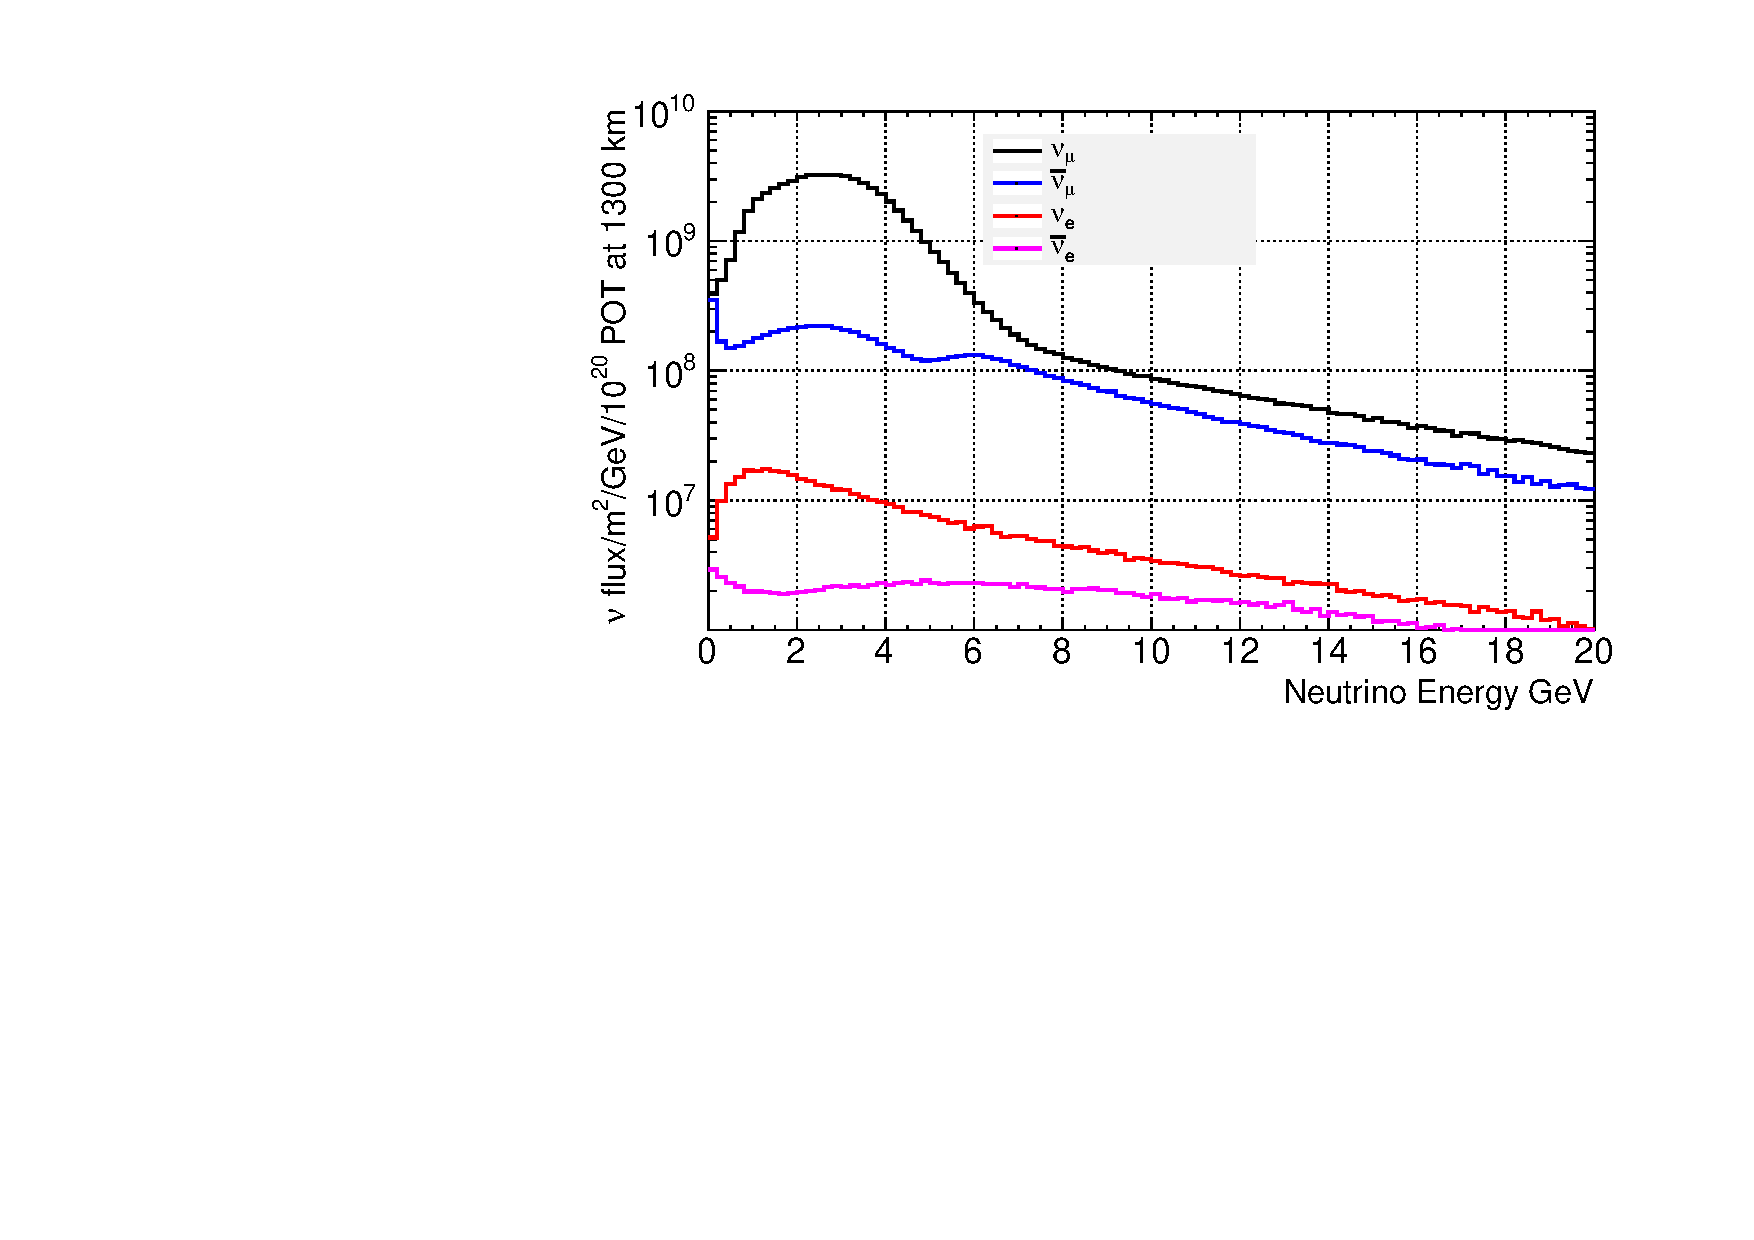
\includegraphics[width=1.0\textwidth]{flux_FHC}
\end{minipage}\hfill 
\begin{minipage}{0.45\textwidth}
\centering 
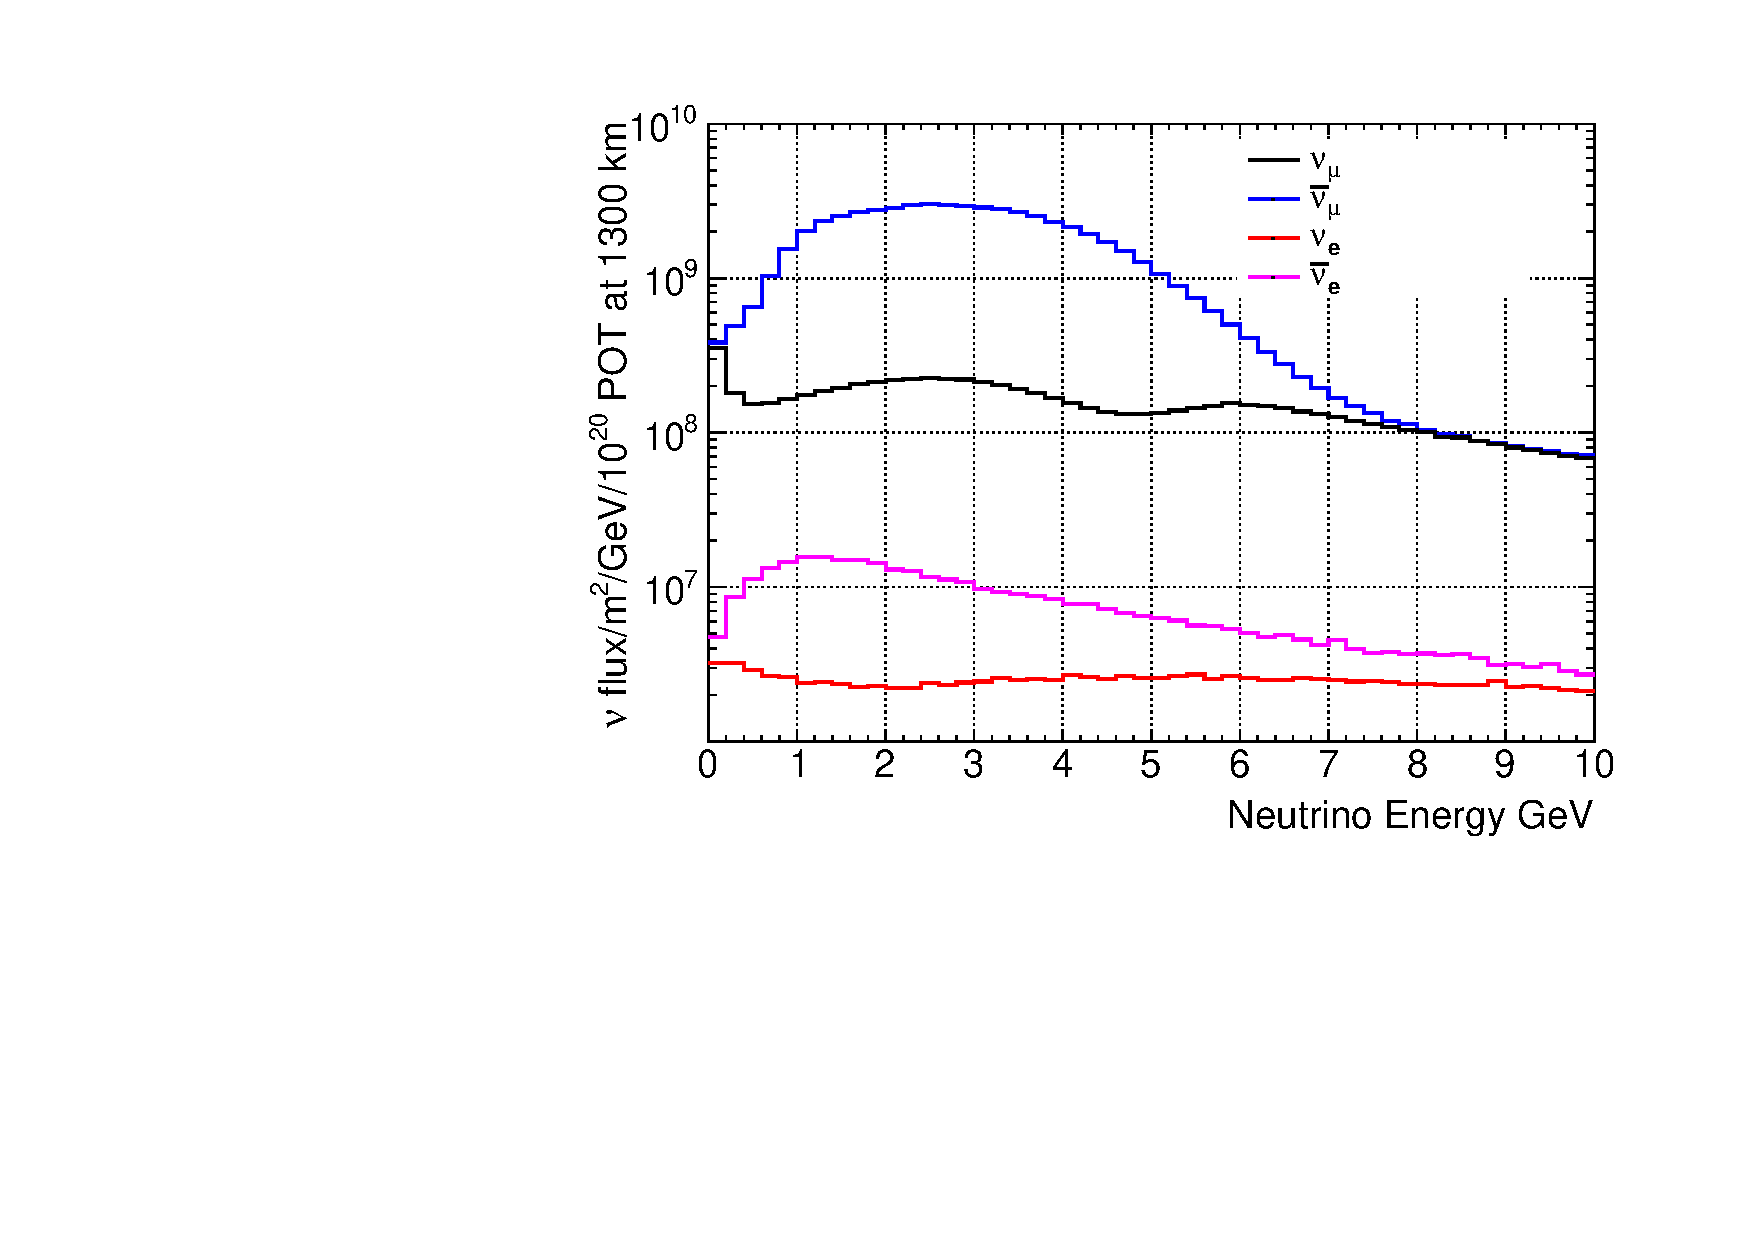
\includegraphics[width=1.0\textwidth]{flux_RHC}
\end{minipage}
\end{cdrfigure}
\begin{cdrfigure}[Neutrino flux comparison for various target
  positions and decay pipe lengths.] {beam_req_lemehe}{Simulated neutrino fluxes for the 
    reference beam design, with the target starting 45 (LE), 135 (ME) 
    and 250 (LE) cm upstream from the start of Horn 1 (left), and the
    fractional improvement in flux for the same beam configurations 
    when the decay pipe is lengthened to 250 m (right).}
    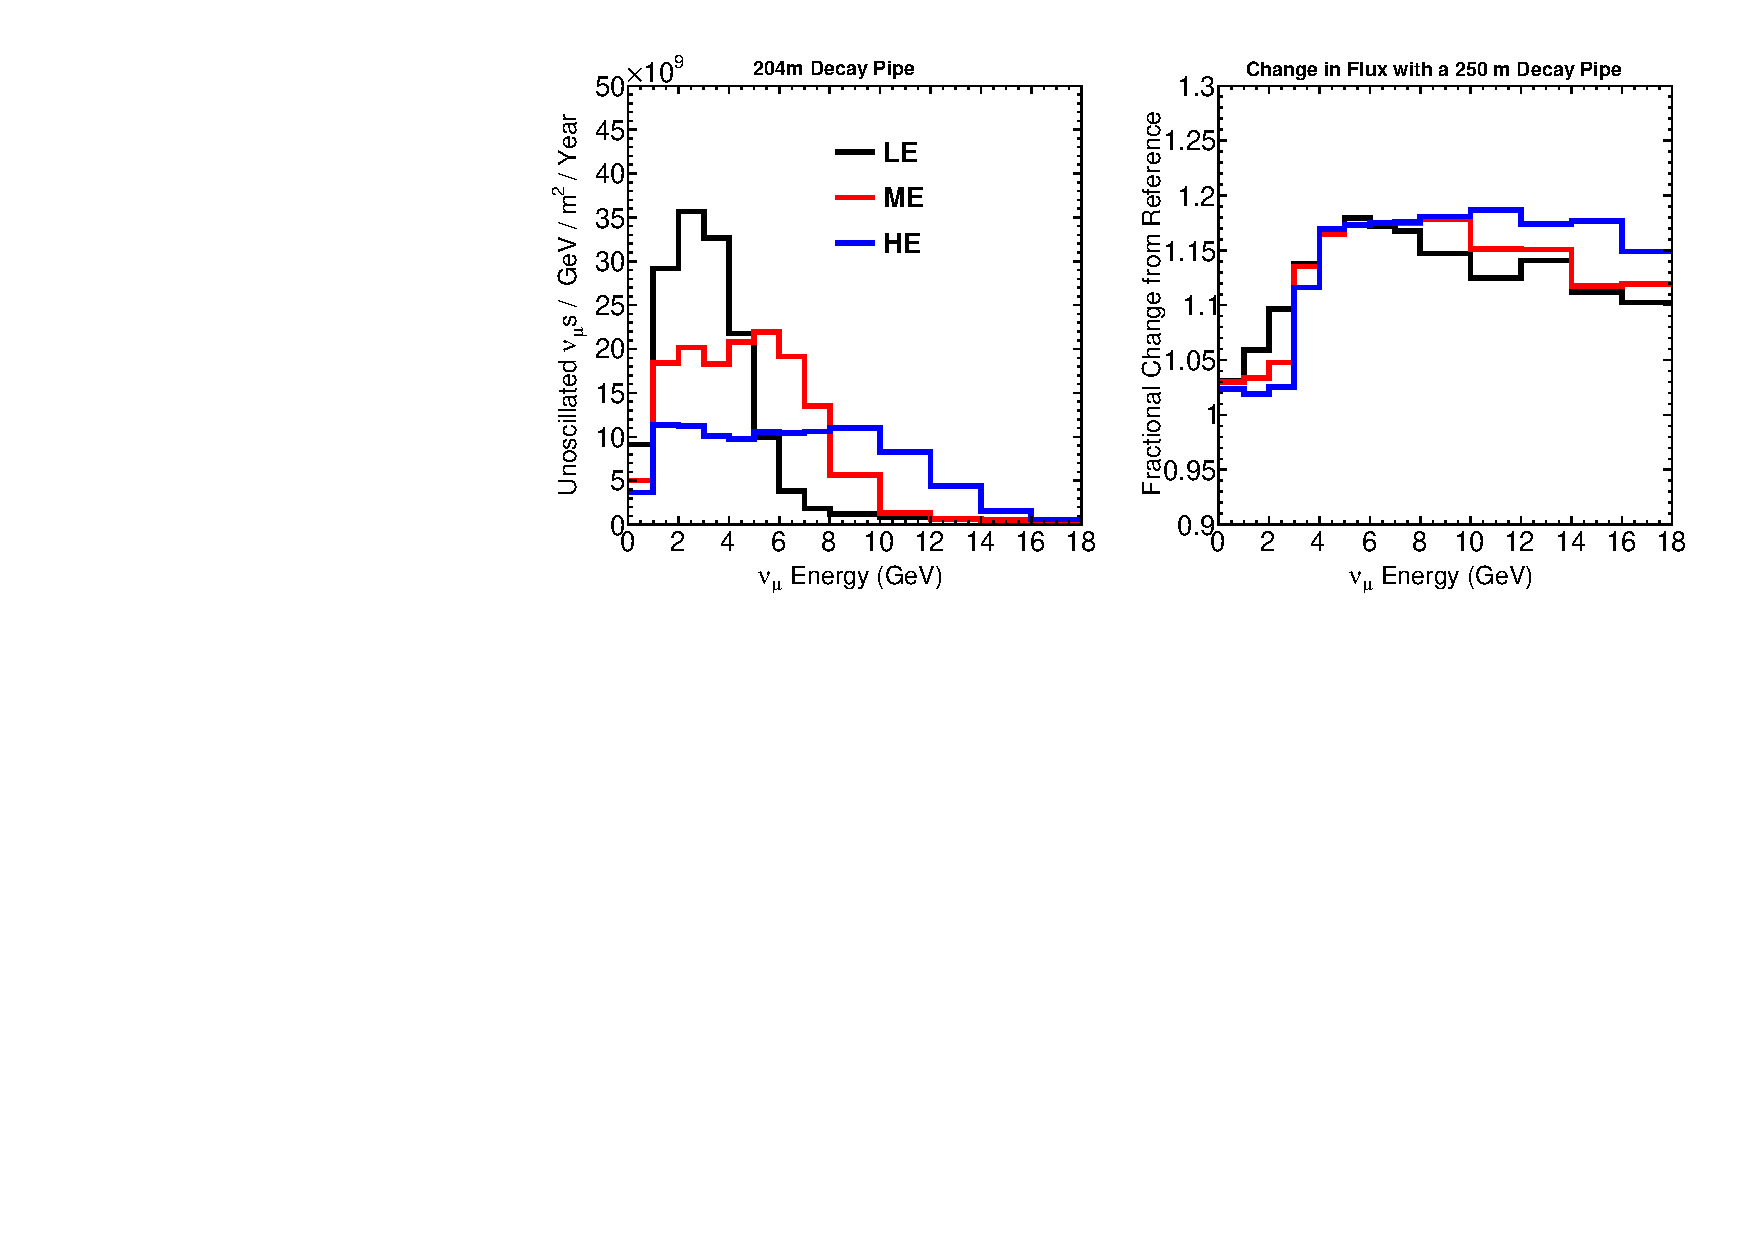
\includegraphics[width=0.75\textwidth]{LEMEHEComp}
  \end{cdrfigure}
\subsection{Alternate Beam Options}
\label{subsec:alternative-focusing-systems}
\begin{cdrfigure}[Radial view of the Horn 1 shape considered in focusing system 
  optimization]{beam_req_opthorn}{Horn 1 design considered 
    in the alternate focusing optimization. \bf{To be replaced with a 
      better drawing}}
  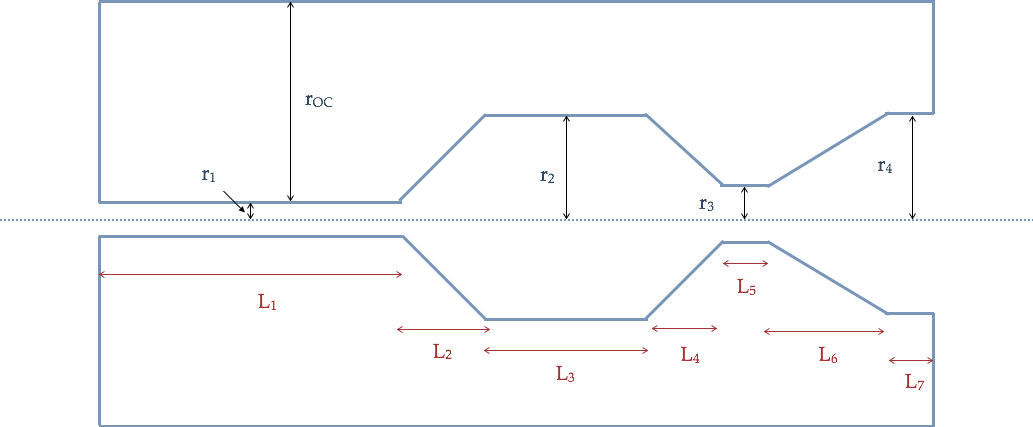
\includegraphics[width=0.75\textwidth]{horn1}
\end{cdrfigure}
There are several potential modifications to the reference beam design would improve the
the experiment's sensitity to the CP violating phase and mass hierarchy.  
The option offering the largest gains in sensitivity is a redesign of 
focusing system, including target, horns and target chase.  To identify optimal
designs, a genetic algorithm was been implemented to search
for beam configurations that maximize sensitivity to CP violation.
The procedure is inspired by a similar one developed by the
LBNO collaboration~\cite{LBNO}, and considers 20 beamline
parameters governing the primary proton energy, target dimensions, and
horn current, positions and shapes.   The optimization parameters,
their allowed ranges and the parameters chosen by the genetic
algorithm, are shown in Table~\ref{tab:beam_req_opt_parameters}.
\begin{cdrtable}[Parameters of focusing system optimization]{ccc}{beam_req_opt_parameters}
{Parameters considered in focusing system optimization.  The first 
  12 govern the shape of Horn 1 (see 
  Figure~\ref{fig:beam_req_opthorn}).  The second focusing horn was 
  constrained to be similar to the NuMI design, modified by radial and 
  longitudinal scale factors and a radial offset.  The target design 
  was also fixed to the NuMI design, with a variable length and 
  width.} 
Parameter &  Allowed Range & Preferred Value \\ \toprowrule  
Horn 1 $r_1$ & 20 - 50 & 38 mm \\  
Horn 1 $r_2$ & 35 - 200 & 162 mm \\  
Horn 1 $r_3$ & 20 - 75 & 54 mm\\    
Horn 1 $r_4$ & 20 - 200 & 167 mm\\  
Horn 1 $r_{OC}$ & 200 - 800 & 670 mm\\  
Horn 1 $l_{1}$ & 800 - 2500 & 1811 mm\\  
Horn 1 $l_{2}$ & 50 - 1000 & 796 mm\\  
Horn 1 $l_{3}$ & 50 - 1000 & 594 mm\\  
Horn 1 $l_{4}$ & 50 - 1000 & 676 mm\\  
Horn 1 $l_{5}$ & 50 - 1000 & 140 mm\\  
Horn 1 $l_{6}$ & 50 - 1000 & 525 mm\\  
Horn 1 $l_{7}$ & 50 - 1000 & 997 mm\\ 
\colhline   
Horn 2 Longitudinal Scale & 0.5 - 2 & 1.32\\   
Horn 2 Radial Scale & 0.5 - 2 & 1.78\\    
Horn 2 Radial Offset & -78 - 100 & 7.6 mm \\ 
Horn 2 Longitudinal Position & 3000 - 15000 & 14400 mm \\
\colhline  
Target Length & 500 - 2500 & 2370 mm \\ 
Target Width & 9 - 15 & 9.74 mm \\
\colhline  
Proton Energy & 40 - 130 & 66 GeV \\ 
Horn Current & 150 - 300 & 297 kA \\
\end{cdrtable} 
There are several modifications to the reference focusing system that  
would increase sensitivity, albeit not as significantly as complete  
redesign.  Lengthening the decay pipe, increasing the current in the  
horns, decreasing the primary proton energy and using a cylindrical  
Beryllium target all improve the neutrino flux in the region of
interest to $\delta_{CP}$ and the mass hierarchy measurements.  A
summary of the flux improvements are described in
Table~\ref{tab:beam_req_reference_options}.
\begin{cdrtable}[Optional flux improvements]{ccc}{beam_req_reference_options}
{Changes in muon neutrino flux (integrated over two energy regions) with several possible upgrades to the
  reference beam.} 
 &  0.5-2 GeV & 2-5 GeV \\ \toprowrule  
84 cm Cylindrical Beryllium Target &  &  \\  
250 m Decay Pipe & 6.4 & 12.5 \\  
230 kA Horn Current & 4.8 & 13.5\\    
80 GeV Proton Beam & 1.4  & -3.9 \\
Total & & \\
\end{cdrtable} 

Figure~\ref{fig:beam_req_focusing_comp} shows a comparison of flux,
signal rates, wrong sign background rates, and sensitivities to $\delta_{CP}$ in
the optimized beam compared to the reference design and an enhanced
version of the reference design.  The optimized focusing system substantially
increases flux in the 0.5-4 GeV region while decreasing wrong sign
contamination.  Assuming an exposure of 150 MW-yr-kton, the net increase in 75\% $\delta_{CP}$ coverage over the reference
design is 27\% ({\bf{to be updated with the latest estimates}}).  Although a mass hierarchy measurement was not
explitly optimized here, the optimized beam improves the minimum
sensitivity to the mass hierarchy by 38\% ({\bf likewise}).   It is
important to note that the optimized beam configuration includes a
second focusing horn that is 32\% longer and 9.8 meters further
downstream than that of the reference focusing design.  These options would require an increase in size of the reference target chase.

\begin{cdrfigure}[Flux, event rates and CP sensitivities of alternate 
  focusing options]{beam_req_focusing_comp}{Neutrino mode muon
    neutrino fluxes (top left), neutrino mode $\nu_e$ signal rates
    (top right),
    antineutrino mode $\nu_e$ background rates (top left) and
    sensitivities to $\delta_{cP}$ for several beams including the
    reference design, the enhanced reference design considered
    throughout this volume, and the optimized beam described in section~\ref{sec:alternative-focusing-systems}}
  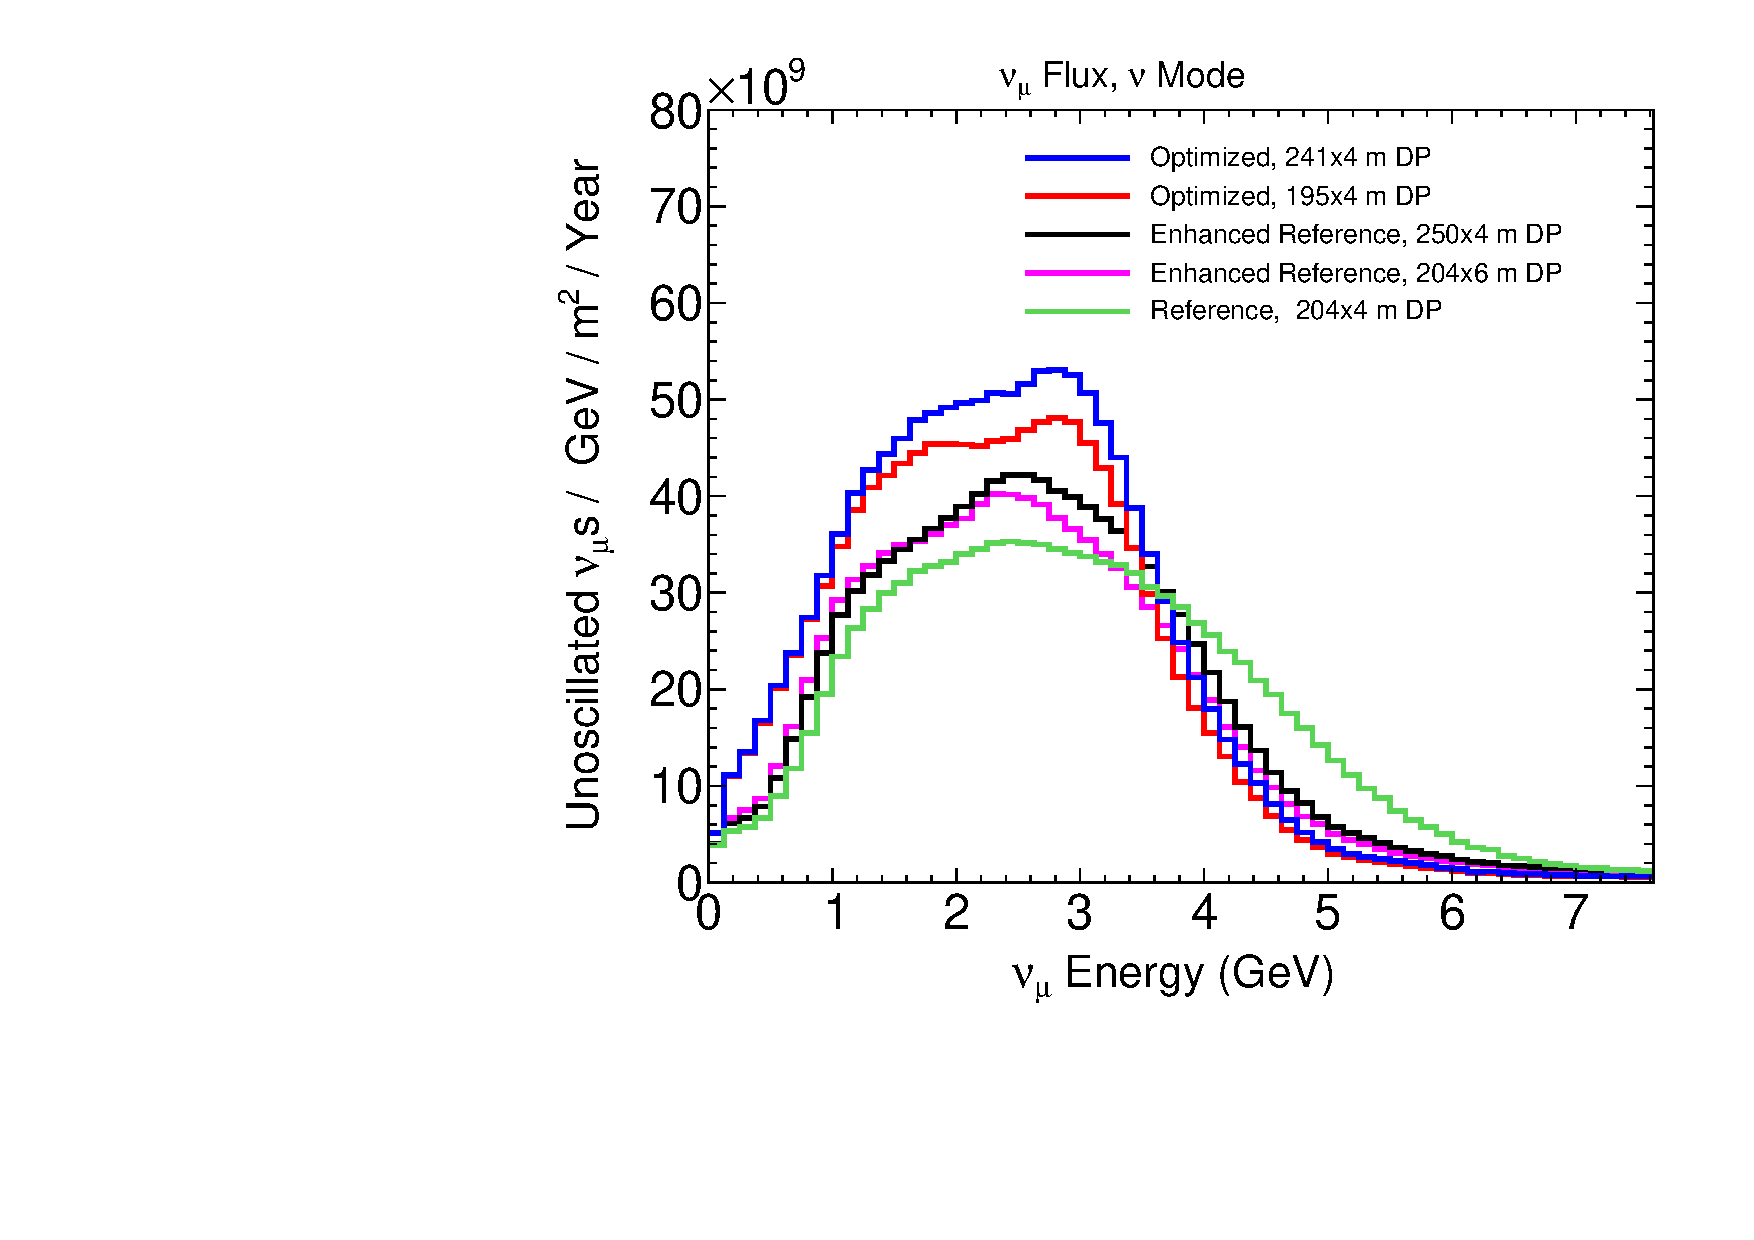
\includegraphics[width=0.66\textwidth]{BeamOptCDR}
\end{cdrfigure}


\section{Far Detector Requirements}
\label{sec:physics-lbnosc-fd-req}

\section{Beam systematic errors and Near Detector Requirements}
\label{sec:physics-lbnosc-beamnd-req}

As described in Section~\ref{sect:globes}, the effect of systematic uncertainty on
experimental sensitivity is approximated using signal and background
normalization uncertainties. In the sensitivities presented here, the
normalization uncertainties on the \numu and \anumu samples are 5\%
on signal and 10\% on background. In this section, we consider the effect of
varying the size of the residual normalization uncertainties
on the \nue and \anue samples, which are 100\% uncorrelated from each other and from the
\numu and \anumu uncertainties.
Figure \ref{fig:exp_systs} shows the
DUNE sensitivity to neutrino mass hierarchy and discovery of CP violation
as a function of exposure for several levels of this uncertainty.

As seen in Fig.~\ref{fig:exp_systs}, for early phases of DUNE
with exposures less than 100 kt-MW-years, the experiment
will be statistically limited. In the full experiment, signal and
background normalization uncertainties remain
relatively unimportant for the mass hierarchy measurement, when considering
minimum sensitivity for 100\% of \deltacp values, because the minimum sensitivity 
occurs in the near-degenerate region where \deltacp is near $\pi/2$. In this
region, much of the sensitivity to mass hierarchy comes from spectral analysis of
the oscillations and is therefore less sensitive to normalization uncertainty.
It is important to note that the sensitivity calculations presented here do not
consider the effect of energy scale uncertainty, which may have a more significant
impact on mass hierarchy sensitivity. Studies of the impact of energy scale 
uncertainty are in progress and will be included in future analyses of experimental
sensitivity. The impact of systematic uncertainty on the CP violation sensitivity
is obvious in Fig.~\ref{fig:exp_systs}; the normalization of the \nue sample,
relative to the \anue, \numu, and \anumu samples after all constraints from
external, near detector, and far detector data have been applied, must be determined 
at the 1-2\% level in order to reach 5$\sigma$ sensitivity for exposures less 
than 900 kt-MW-years.
% \begin{figure}[!htbp]
% \centering
% \includegraphics[width=0.45\linewidth]{figs/MHSigFrac_lbne_SBGErrs.pdf}
% \includegraphics[width=0.45\linewidth]{figs/CPVSigFrac_lbne_SBGErrs.pdf}
% \caption{Expected sensitivity of DUNE to determination of the neutrino mass
%   hierarchy (left) and discovery of CP violation, i.e. $\dcp \ne$ 0 or $\pi$,
%   (right) as a function of exposure in kt-MW-years, assuming 
%   equal running in neutrino and antineutrino mode, for a range of values for
%   the residual \nue and \anue signal and
%   background normalization uncertainties. The sensitivities quoted
%   are the minimum sensitivity for 100\% of \deltacp values in the case of 
%   mass hierarchy and 50\% of \deltacp values in the case of CP violation.
%   Sensitivities are for true normal hierarchy; neutrino mass hierarchy is assumed to
%   be unknown in the CPV fits.}
% \label{fig:exp_systs}
% \end{figure}

Uncertainties in DUNE
will be constrained by external data, near detector data, and the combined
fit to the four (\nue, \anue, \numu, \anumu) far detector samples.  
Experience from previous and currently-running neutrino oscillation 
experiments suggests that 1-2\% uncertainty in uncorrelated $\nu_e$
signal normalization and 5\%
uncorrelated uncertainty in background normalization for the 
$\nu_e$-appearance measurement
is reasonably achievable in DUNE given a capable near detector.
Table~\ref{tab:nuesysts} shows the uncertainties in a \nue appearance
analysis achieved by MINOS~\cite{Adamson:2013ue} 
and T2K~\cite{Abe:2013hdq} and compares the 
expected uncertainty in
DUNE. The projected uncertainties in DUNE are chosen by determining which
of the existing experiments is more representative of DUNE for each source
of systematic uncertainty and then setting the reasonable goal that a next
generation experiment, with the high resolution of a LArTPC and precise measurements
from a highly capable near detector, should be able to improve on a similar earlier experiment.
Based on this exercise, the \emph{total} uncertainty on the \nue sample in
DUNE is expected to be less than 4\%; significant cancellation of uncertainty
is expected in the four-sample fit, so the residual uncorrelated uncertainty 
is expected to be reduced to the 1-2\% level.
\begin{table}[!hb]
\begin{center}
  \caption {The dominant systematic uncertainties on the $\nu_e$-appearance 
    signal prediction in MINOS and T2K and a conservative projection of the 
    expected uncertainties in DUNE. In each case, the quoted uncertainty is
    the effect on the $\nu_e$-appearance signal only. These uncertainties 
    are the \emph{total} expected uncertainties on the $\nu_e$-appearance signal 
    which include both correlated and uncorrelated uncertainties in the 
    three-flavor fit.\vspace{2pt}}
\label{tab:nuesysts}
\begin{tabular}{|l|c|c|c|l|} \hline\hline
Source of & MINOS & T2K & DUNE & Comments \\ 
Uncertainty & $\nu_e$ & $\nu_e$ & $\nu_e$ & \\ \hline\hline
Beam Flux & 0.3\% & 2.9\% & 2\% & MINOS is normalization only.\\ 
after N/F & & & & DUNE normalization  and shape   \\
extrapolation & & & & highly correlated between $\nu_\mu/\nu_e$. \\ \hline\hline
\multicolumn{5}{|c|}{Neutrino interaction modeling}  \\ \hline
Simulation & 2.7\% & 7.5\% & $\sim 2\%$ & Hadronization models are better  \\
includes: & & & & constrained in the DUNE LArTPC. \\
hadronization & & & &  N/F cancellation larger in MINOS/DUNE. \\ 
cross sections & & & & X-section uncertainties larger at T2K energies. \\ 
nuclear models & & & & Spectral analysis in DUNE provides \\ 
& & & & extra constraint. \\ \hline\hline
\multicolumn{5}{|c|}{Detector effects}  \\ \hline
Energy scale  & 3.5\% & included& (2\%) & Included in DUNE $\nu_\mu$ sample  \\ 
($\nu_\mu$) & & above & &  uncertainty only in 3-flavor fit. \\
& & & & MINOS dominated by hadronic scale. \\ \hline
Energy  scale & 2.7\% & 3.4\% & 2\% & Totally active LArTPC with calibration \\
($\nu_e$) & & includes & & and test beam data lowers uncertainty. \\
 & & all FD & & \\
 & & effects & & \\ \hline 
Fiducial & 2.4\% & 1\% & 1\% & Larger detectors = smaller uncertainty. \\ 
volume & & & & \\ \hline\hline
Total  & 5.7\% & 8.8\% & 3.6 \% & Uncorrelated $\nu_e$ uncertainty in  \\ 
& & & & full DUNE 3-flavor fit = 1-2\%. \\ \hline\hline
\end{tabular}
\end{center}
\end{table}
%
Detailed determination of expected systematic uncertainty using DUNE-specific
simulations and tools is a high priority of the collaboration and is in progress.
Detailed description of this effort is beyond the scope of this document; only
a brief summary of preliminary results will be presented here. 

As described in
Section~\ref{sect:neardetector}, 
{\bf Note:I assume this will be discussed in ND section}
initial studies using a Fast Monte Carlo with a parameterized detector response
predict 2-3\% statistical uncertainties on the absolute flux using fully 
leptonic neutrino interactions for which high-precision cross-section predictions 
exist. Specifically,
the statistical uncertainty is expected to be 2\% for neutrino-electron
scattering ($E_\nu<5$~GeV) and 3\% for inverse muon decay ($E_\nu>11$~GeV).
Relative normalization using the low-$\nu_0$ method is
expected to constrain the flux shape and the near/far flux ratio to 1-2\%.
Studies using a multi-sample fit  to constrain the flux with simulated near detector
event samples show significant constraints on all flux
uncertainties. The post-fit uncertainty 
in most flux bins for a preliminary fit is less
than 5\%, which is the uncorrelated \numu signal normalization
uncertainty assumed by the sensitivity calculations. 

Results from a fit to Fast MC simulation of all four far detector samples
(\nue, \anue, \numu, \anumu) significantly
constrains cross-section systematic uncertainty even in the case where many
cross-section parameters are allowed to vary simultaneously within their
GENIE uncertainties. As seen in the example shown in Figure
\ref{fig:MAresqesyst}, 
a fit in which both $M_A^{QE,CC}$ and 
$M_A^{RES,CC}$ are allowed to vary within their GENIE uncertainties 
($\pm$20\%), which could significantly alter the energy distribution of the 
the selected events, results in a dramatic reduction in sensitivity if one 
considers only the $\nu_e$ appearance signal without constraint from the 
$\bar{\nu}_e$ and $\nu_{\mu}$/$\bar{\nu}_{\mu}$ samples.
In contrast, for a four sample fit,
this same parameter variation results in only a small reduction in
sensitivity to CP violation.
This result includes a 10\% uncertainty in the $\nu/\bar{\nu}$
cross-section ratio and a 2.5\% uncertainty in the $\nu_e/\nu_{\mu}$
cross-section ratio.
Preliminary studies also
demonstrate significant constraint on cross-section systematics from the 
near detector. The validity of the GENIE model parameter uncertainties are being studied 
via comparisons with available data (e.g. MINERvA), and alternate models (e.g. the 
Intranuke intranuclear recattering model will be compared with GiBUU). These comparisons 
are a high priority of the whole neutrino community as well as the DUNE collaboration.
% \begin{figure}[!htbp]
% \centering
% 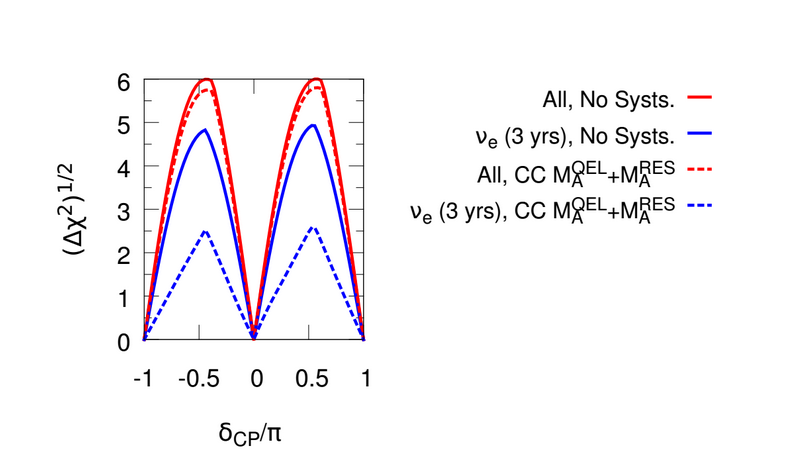
\includegraphics[width=0.8\linewidth]{figs/CPV_MARESQE.png}
% \caption{An example CP violation sensitivity calculated using inputs from the 
%   FastMC in a fit to all four ($\nu_e$, $\overline\nu_e$, $\nu_{\mu}$, 
%   $\overline\nu_{\mu}$) samples (red) and a fit to the $\nu_e$ appearance sample 
%   only (blue), for the case of no systematic uncertainty (solid) and the case in
%   which both $M_A^{QE,CC}$ and $M_A^{RES,CC}$ are allowed to vary with a
%   1$\sigma$ uncertainty of 20\% (dashed). This example was taken from an earlier
%   DUNE study, so the absolute sensitivity can not be compared with the DUNE 
%   sensitivities presented in this document.}
% \label{fig:MAresqesyst}
% \end{figure}

Uncertainty from nuclear interactions, in which particles exiting the primary
interaction vertex interact with the nuclear medium prior to depositing energy
in the detector, and detector effects, such as resolutions and energy scale
uncertainty, are somewhat more difficult to address with early simulation efforts.
However, in analogy to the treatment of cross-section uncertainty described above,
the effect of varying nuclear interaction parameters within their GENIE
uncertainties and comparisons of GENIE predictions to those of other
event generators are in progress.
Efforts to improve modeling of nuclear interactions and to develop 
reconstruction and analysis tools for a full Monte Carlo simulation are also underway. 
At the same time,
a number of test-beam and prototype experiments, including the DUNE 35-t prototype,
LARIAT, CAPTAIN, and the CERN neutrino platform experiments, 
{(\bf More details here or less?)} are being designed and built to reduce these
uncertainties with experimental data.

